\documentclass[sigconf,nonacm]{acmart}
\usepackage{booktabs,tabularx,tikz,listings,xurl}
\usetikzlibrary{positioning,arrows.meta,fit,calc}
\settopmatter{printacmref=false,printccs=false,printfolios=true}
\renewcommand\footnotetextcopyrightpermission[1]{}
\setcopyright{none}
\DeclareUrlCommand\code{\urlstyle{tt}}
\emergencystretch=1.5em
\newcommand{\M}{MorletDB}
\lstset{basicstyle=\ttfamily\footnotesize,columns=fullflexible,keepspaces=true,frame=tb,framerule=0.4pt,
  morekeywords={SELECT,FROM,WHERE,AS},keywordstyle=\bfseries,aboveskip=4pt,belowskip=4pt}

\begin{document}
\title{Supplement to ``MorletDB: Recordings, Not Rows''}
\subtitle{Working draft 0.8 --- not for distribution}
\author{Zin Nam}
\affiliation{\institution{}\country{}}
\maketitle
\section*{About this supplement}
This supplement holds studies that support the system described in the main paper but are not needed for its argument: lossless storage of raw samples, envelope precision, building representations outside or inside the database, access control, recovery and load tests, and application evidence and negative results. Text, tables and numbers are carried over from draft 0.6 of the paper; protocols and raw results are in the repository~\cite{repo}. Section and table references to ``the paper'' refer to the main manuscript.

The machine, PostgreSQL and pgvector versions are those of the main paper. TimescaleDB 2.30.2 ran in Docker; we compare its sizes, not its speed.

\section{Lossless chunk coding}\label{sec:codec}
Each raw chunk is one \code{bytea} value. The codec combines established techniques: fixed polynomial predictors of order 0--4 as in Shorten and FLAC~\cite{shorten,flac}, partitioned Rice coding of zig-zag mapped residuals~\cite{rice}, and a CRC-32C checksum. Its distinctive part is how it treats floats.

Most sensor values are calibrated integers: a digitizer emits counts $d$, and acquisition software stores $x=f(d)$, for example $x=d\cdot s$ (seismic counts, WAV) or, in EDF~\cite{edf}, $x=(d-d_{\min})(p_{\max}-p_{\min})/(d_{\max}-d_{\min})+p_{\min}$. The recording declares a nominal quantum $q$: 1 for counts, 0.001 for three decimals, the ADC step for calibrated values. Per chunk, the encoder seeks a grid
\begin{equation}
x_i \;=\; o + k_i\,s \;\oplus\; \delta_i,
\end{equation}
with integer indices $k_i$, a step $s$ refined from $q$ to within one unit in the last place (ulp), an offset $o$ (format version 3; zero in version 2), and corrections $\delta_i$, stored as differences of order-preserving integer images of float64, so that decoding reproduces every bit pattern. A division mode $x=k/d$ covers decimal steps exactly. Indices are predicted and Rice-coded like integers; corrections form a second stream. If no grid fits within a thousandth of a step, the chunk is coded as order-preserving float bits, and if that is not smaller, as raw float64. The quantum is a storage hint, never a conversion: a wrong quantum costs space, not accuracy.

\section{Storage of raw samples}\label{sec:storage}
\subsection{Database footprint (P2)}
P2 appended the same 4,194,304 samples of four inputs (CX seismic counts~\cite{ipoc}, IMS bearing vibration~\cite{ims}, Paderborn bearing vibration~\cite{paderborn} as ADC counts and as physical floats) to \M{} and to TimescaleDB hypertables with native compression (Gorilla for floats; delta-of-delta and Simple-8b for integers), and measured total on-disk bytes, including indexes, TOAST and metadata tables, after verifying that four intervals per layout read back bit-exactly~\cite{plain}.

\begin{table}[t]
\caption{P2: total database storage in bits per sample. T: the TimescaleDB layouts tested (a row per sample with an integer or float column; a row per 4096-sample array).}
\label{tab:p2}
\small
\begin{tabular}{@{}lrrrr@{}}
\toprule
Input & \M{} & T int & T float & T array \\
\midrule
CX seismic counts & \textbf{6.12} & 8.25 & 14.34 & 25.0 \\
IMS three-decimal & \textbf{11.36} & 14.06 & 71.95 & 28.1 \\
Paderborn counts & \textbf{9.95} & 12.89 & 24.58 & 26.4 \\
Paderborn physical & \textbf{11.53} & --- & 70.12 & 29.5 \\
\bottomrule
\end{tabular}
\end{table}

TimescaleDB on integer columns comes closest but is 24--35\% larger (Table~\ref{tab:p2}), and requires the user to convert values to counts first. On float columns, Gorilla's XOR coding \emph{expands} noisy decimal and calibrated values beyond 64 bits per sample. We tested one \code{segmentby}/\code{orderby} configuration and not TimescaleDB's newer column formats. Of \M{}'s footprint, the codec payload is 4.6--9.2 bits per sample (Table~\ref{tab:b1}); PostgreSQL row and TOAST overhead adds 1.5--2.6 bits per sample at 4096-sample chunks.

\subsection{Codec against modern baselines (B1)}
B1 compares codecs on identical samples, each verified lossless~\cite{b1}. Float codecs receive only float64 values: zstd level 19 per chunk, Parquet with \code{BYTE_STREAM_SPLIT} and zstd, and DuckDB 2.0's automatic float compression, which uses ALP and its fallback ALP-RD~\cite{alp,duckdb}. \M{} receives the values plus the nominal quantum. Integer codecs receive the exact digitizer counts: FLAC~\cite{flac}, Parquet delta coding with zstd, and DuckDB bit-packing. Two inputs extend the earlier storage inputs: a Sleep-EDF EEG slice~\cite{sleepedf,physionet} from 32 nights with symmetric and asymmetric calibration ranges (an earlier engineering check had measured \M{}'s own storage of this collection, not the other arms), and PTB-XL ECG lead~I~\cite{ptbxl}, new to the storage studies. The Parquet float arm is one fixed encoding, not a tuned Parquet baseline; ALP is DuckDB 2.0.0's implementation, measured as table blocks.

\begin{figure}[t]
\centering
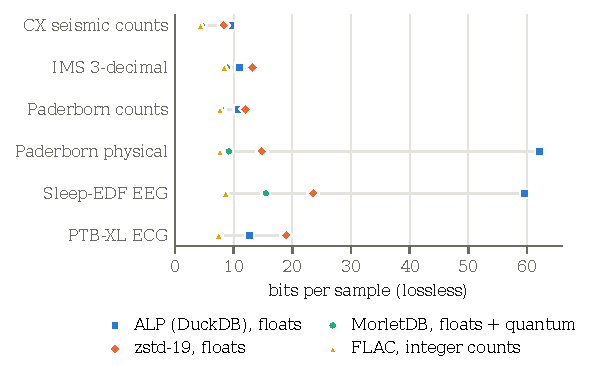
\includegraphics[width=\linewidth]{fig/storage.pdf}
\caption{B1: lossless bits per sample on identical samples. Float codecs see only float64 values; \M{} also sees the nominal quantum; FLAC sees integer counts. Table~\ref{tab:b1} gives all arms.}
\label{fig:storage}
\end{figure}

\begin{table}[t]
\caption{B1: bits per sample. Z: zstd-19; PQ: Parquet; DDB: DuckDB.}
\label{tab:b1}
\small\setlength{\tabcolsep}{2.7pt}
\begin{tabular}{@{}lrrrr|rrr@{}}
\toprule
& \multicolumn{4}{c|}{float input} & \multicolumn{3}{c}{integer input} \\
Input & Z & PQ & ALP & \textbf{\M{}} & FLAC & PQ & DDB \\
\midrule
CX counts & 8.33 & 6.84 & 9.50 & \textbf{4.61} & 4.38 & 5.24 & 6.38 \\
IMS 3-decimal & 13.24 & 42.94 & 11.00 & \textbf{8.81} & 8.41 & 9.87 & 10.88 \\
Paderborn counts & 12.04 & 9.48 & 10.75 & \textbf{7.88} & 7.70 & 9.61 & 11.25 \\
Paderborn physical & 14.82 & 30.57 & 62.13 & \textbf{9.17} & 7.70 & 9.61 & 11.25 \\
Sleep-EDF EEG & 23.54 & 38.15 & 59.63 & \textbf{15.51} & 8.65 & 10.22 & 12.00 \\
PTB-XL ECG & 18.94 & 44.64 & 12.75 & \textbf{7.40} & 7.46 & 10.27 & 12.75 \\
\bottomrule
\end{tabular}
\end{table}

Figure~\ref{fig:storage} and Table~\ref{tab:b1} show three regimes.

\emph{Counts and decimals.} When values are integers or short decimals (CX, IMS, Paderborn counts, ECG with gain 1000), ALP and \M{} both recover integers; \M{} is 20--51\% smaller than ALP, plausibly because consecutive samples are correlated and prediction exploits that, while ALP's frame-of-reference bit-packing does not; B1 does not isolate this. \M{} is within 5\% of FLAC, whose LPC stage it lacks, and slightly below FLAC on ECG.

\emph{Calibrated floats.} On Paderborn physical values and Sleep-EDF, no decimal exponent turns values into integers, and the tested DuckDB ALP implementation selected ALP-RD, storing about 60 bits per sample, near raw. Of the three metadata-free arms, zstd was smallest. \M{}, which additionally receives the nominal quantum, was 1.5--1.6$\times$ smaller than zstd. Our pre-registered claim of at least 2$\times$ was not met.

\emph{The correction gap.} Given counts, \M{} codes the two calibrated inputs at 7.9 and 8.8 bits per sample; given the calibrated floats, it needs 1.3 and 6.7 bits per sample more. That extra cost, relative to \M{}'s own integer-input path, is the correction stream: the source software computed $x$ with a particular sequence of roundings (on Sleep-EDF a multiplication, a division and an addition), which a single fitted step and offset does not reproduce for every sample. It does not explain the whole difference from FLAC, which also includes \M{}'s integer path being 0.15--0.18 bits per sample larger than FLAC's. Replaying the source's calibration arithmetic might remove the corrections when the correct parameters and operation sequence are known; this is neither implemented nor tested. Our pre-registered claim that \M{} stays within 15\% of the best integer codec held on four of six inputs and failed on these two.

For float compression, these inputs illustrate that real-valued sensor data can be neither decimal nor arbitrary but an affine image of integers under floating-point rounding. On the two such inputs we tested, the decimal-oriented ALP implementation fell back to near-raw size and the best byte-oriented arm was 1.5--1.6$\times$ larger than coding with a declared quantum.

\section{Envelope precision and zero-lag storage (R1b, P1)}
\subsection{Precision of materialized envelopes (R1b)}
R1b selected an envelope precision on 2023 seismic windows and evaluated it once on 2022 event and noise windows that, according to its report, no earlier study had read: 1,826 windows at ten CX stations~\cite{ipoc}, 1,557 event windows from 284 catalogued events and 269 no-match distractors~\cite{r1b}. The reference decodes raw samples and computes envelopes in the client.

\begin{table}[t]
\caption{R1b on 2022 windows. Size relative to the raw chunk table; latency includes the client path.}
\label{tab:r1b}
\small\setlength{\tabcolsep}{4pt}
\begin{tabular}{@{}lrrrr@{}}
\toprule
Envelopes & Size/raw & Recall@10 & Same order & p95 ms \\
\midrule
from raw (reference) & --- & 1 & 1 & 1324 \\
float32 & 28.1\% & 1.000 & 1.000 & 14 \\
\textbf{float16} & \textbf{12.9\%} & \textbf{0.9999} & \textbf{0.987} & \textbf{16} \\
uint8 & 7.2\% & 0.998 & 0.845 & 17 \\
uint8, coarser & 4.2\% & 0.952 & 0.067 & 16 \\
\bottomrule
\end{tabular}
\end{table}

Float16 envelopes met all frozen criteria (Table~\ref{tab:r1b}): recall@10 of 0.9999, 12.9\% of the raw table, and an unchanged catalogue-distance relevance proxy ($+0.001$\,km, 95\% interval $[-0.002, +0.004]$). The roughly 80-fold latency reduction measures materialization against a client that decodes and recomputes; it is not a speedup over an optimized raw-scanning engine.

\subsection{Same storage, different query (P1)}
P1 stored the identical float16 envelopes in a pgvector \code{halfvec(410)} column~\cite{pgvector}. Both tables occupied exactly 1,794,048 bytes, and all 1,826 envelopes were bit-identical, so envelope storage itself is no advantage. Zero-lag cosine search, however, shared only 64.7\% of the lag-tolerant top ten and reproduced its order for 0.1\% of queries. Scoring lags in the client on the same \code{halfvec} rows reproduced \M{}'s ranking exactly. In a later same-run comparison, median latency was 6.85\,ms for \M{}, 0.49\,ms for zero-lag cosine and 20.3\,ms for client lag scoring. The first two answer different questions, so their ratio is not a like-for-like speed comparison.

\section{Building representations (CW1)}\label{sec:cw1}
As a first step toward compaction-style workers that run representation work outside the database, CW1 compared building envelopes inside PostgreSQL with stateless external processes that read encoded chunks through SQL, compute with the same Rust code, and write rows back with key-idempotent inserts~\cite{cw1}. On 33,736 windows the external path produced byte-identical rows in every run, survived a killed and restarted worker and two workers processing the same recordings, and moved 90\% of the per-window CPU off the database server (0.13 against 1.31\,ms of database CPU per window). It also used about four times less CPU in total, which exposed the real inefficiency: the in-database builder issued one SQL statement per window and decoded every raw sample twice. Batching the in-database builder, so that each chunk is decoded once for up to 256 windows, reduced database CPU to 0.31\,ms per window and raised one session from 740 to 3,084 windows per second (four sessions: 12,034), byte-identical to before. External workers remain a viable basis for separating compute from storage, but on one machine batching delivered most of their benefit without them.

\section{Access control, recovery and load}\label{sec:ops}
Before a bounded pilot with human review of results, we tested access control, recovery and sustained load against plans frozen before each run~\cite{pilot}. All runs shared the machine with an unrelated CPU-intensive job (load average 3--20), so latencies are indicative; correctness results are not affected.

\textbf{Access control.} With row-level security only on the recordings table, a tenant could still read other tenants' chunks, envelopes and probe vectors by querying the companion tables directly: search functions honoured the policy, the tables did not. \code{morlet\_enable\_row\_security} now applies a policy to every companion table that admits rows whose recording is visible. Its first form, a correlated \code{EXISTS}, prevented parallel plans and tripled exact search time (946 to 2,821\,ms on 235,000 windows); comparing against an array of visible recording identifiers kept the parallel scan (995\,ms, $+5\%$) and cost probe search 6\,ms. We did not test policies with thousands of visible recordings.

\textbf{Recovery.} On a 50,604-window database every check passed: each recording hashed identically afterwards, each complete window had exactly one envelope and probe row, and exact searches returned identical lists. A full dump restored in 18\,s; dumping only recordings and chunks took a third of the space (146 against 459\,MB), and rebuilding envelopes and the probe index after restore took 23\,s. Twenty backends terminated at random points inside append transactions left no partial rows, and replaying the chunk succeeded; aborted builds resumed, and an aborted probe enable could be retried. Killed and duplicated external workers produced exactly one byte-identical row per window, but did not write probe rows, so their windows stayed invisible to probe search until filled. After deleting 15\% of recordings, \code{VACUUM} took 113\,s and left the index size unchanged, whereas an online \code{REINDEX} \code{CONCURRENTLY} took 10\,s while four clients searched (p95 23 to 31\,ms). An extension update forced to fail midway rolled back completely.

\textbf{Sustained load.} On an archive of 938,768 windows (4.8\,GB), sixteen channels at 25.6\,kHz (409,600 samples/s) were appended by four writers, each building envelopes and probe rows in the append transaction, while four analysts issued one query every two seconds, half filtered to about 2\% of windows and half unfiltered. With PostgreSQL's default configuration the run met its criteria (filtered p95 167\,ms; probe p95 337\,ms, spot-check recall 0.998; ingest lag at most 22\,s, recovered), but wrote 13.8\,GB of write-ahead log for 0.76\,GB of database growth in 15 minutes: HNSW insertions touch pages across a 1.2\,GB index, and each checkpoint forces full-page images of them. At twice the rate the writers fell behind without recovering; capacity was about 1.3--1.4$\times$ the target. With a pilot configuration (8\,GB shared buffers, 16\,GB \code{max\_wal\_size}, 15-minute checkpoints, WAL compression, changed together) the same run wrote 1.91\,GB of WAL for 0.65\,GB of growth, kept ingest lag at or below 2\,s, and gave filtered and probe p95 of 81 and 100\,ms (recall 0.994); background load was lower in this run (7.3 against 11.7), which confounds the latency comparison but not the WAL volume. Unfiltered exact search over the full archive stayed at 7.8--9.7\,s p95, which is why the router sends large galleries to probes. A run planned for two hours with the same configuration met the target for 111 minutes (409,585 samples/s; writer lag at most 24\,s in the first hour, with the unrelated job running, and 3.4\,s in the second; filtered and probe p95 118 and 138\,ms, recall 0.993; no errors; 12.0\,GB of WAL for 4.7\,GB of growth). Then all client processes paused for 90--106\,s without an error in the server log, and the harness's lag rule, stricter than the protocol's wording, stopped the run at 112.5 minutes; the stored result divides the ingest rate by the scheduled duration, and a re-analysis from the raw logs reports the rate over the elapsed time. The two-hour run therefore did not complete. A measured stability duration is not a production qualification.

\section{Application evidence and negative results}\label{sec:negative}
\textbf{Sleep staging by example (S1).} On 153 Sleep-EDF nights with a subject-disjoint split, staging each 30-second epoch by the 40 most similar expert-scored epochs from other subjects gave a mean per-subject Cohen's $\kappa$ of 0.583, against 0.541 for logistic regression on the same features ($+0.042$, 95\% CI $[0.016, 0.068]$), with equal macro-F1~\cite{sleep}. Retrieval thus exposes source-linked neighbours at no measured accuracy cost against this simple comparator; part of the $\kappa$ difference comes from the regression's class-balanced weights. The result is far from state-of-the-art staging and makes no clinical claim.

\textbf{Morlet versus FFT.} In the same study, FFT band powers with the same band layout gave $\kappa$ 0.589 against 0.583 for Morlet energies. We found no advantage for the wavelet representation and made the extractor replaceable.

\textbf{Wavelet and progressive storage.} A compression benchmark found the tested wavelet decomposition codec 19--57\% \emph{larger} than scalar quantization with conventional coding at matched error bounds, and progressive raw storage missed its byte-saving gate (0.59 against $\le 0.5$ of a cascade) because a separate envelope index dominated~\cite{compression}. This motivated storing a retrieval representation \emph{next to} losslessly coded raw data rather than a multiresolution raw format.

\textbf{Reference coding.} Coding a machining recording as a residual against an earlier execution of the same operation would have saved at most 0.0019\% on the Bosch CNC data~\cite{bosch}, because executions were too dissimilar sample by sample~\cite{x1}.

\textbf{Out of scope.} Three later studies tested retrieval-based forecasting of bearing and turbofan degradation and current-to-vibration estimation; none passed its gate~\cite{repo}. They concern analytics on top of the store rather than storage and retrieval.


\begin{thebibliography}{40}\small
\bibitem{alp} Azim Afroozeh, Leonardo X. Kuffo, and Peter Boncz. 2023. ALP: Adaptive Lossless floating-Point Compression. \emph{Proc. ACM Manag. Data} 1, 4, Article 230 (Dec. 2023), 26 pages. doi:10.1145/3626717.
\bibitem{fcbench} Xinyu Chen, Jiannan Tian, Ian Beaver, Cynthia Freeman, Yan Yan, Jianguo Wang, and Dingwen Tao. 2024. FCBench: Cross-Domain Benchmarking of Lossless Compression for Floating-Point Data. \emph{Proc. VLDB Endow.} 17, 6 (2024), 1418--1431. doi:10.14778/3648160.3648180.
\bibitem{gorilla} Tuomas Pelkonen, Scott Franklin, Justin Teller, Paul Cavallaro, Qi Huang, Justin Meza, and Kaushik Veeraraghavan. 2015. Gorilla: A Fast, Scalable, In-Memory Time Series Database. \emph{Proc. VLDB Endow.} 8, 12 (2015), 1816--1827. doi:10.14778/2824032.2824078.
\bibitem{chimp} Panagiotis Liakos, Katia Papakonstantinopoulou, and Yannis Kotidis. 2022. Chimp: Efficient Lossless Floating Point Compression for Time Series Databases. \emph{Proc. VLDB Endow.} 15, 11 (2022), 3058--3070. doi:10.14778/3551793.3551852.
\bibitem{shorten} Tony Robinson. 1994. SHORTEN: Simple lossless and near-lossless waveform compression. Technical Report CUED/F-INFENG/TR.156, Cambridge University Engineering Department.
\bibitem{flac} Martijn van Beurden and Andrew Weaver. 2024. Free Lossless Audio Codec (FLAC). RFC 9639, RFC Editor. doi:10.17487/RFC9639.
\bibitem{rice} Robert F. Rice. 1979. Some Practical Universal Noiseless Coding Techniques. JPL Publication 79-22 (NASA-CR-158515), Jet Propulsion Laboratory.
\bibitem{edf} Bob Kemp, Alpo V\"arri, Agostinho C. Rosa, Kim D. Nielsen, and John Gade. 1992. A simple format for exchange of digitized polygraphic recordings. \emph{Electroencephalography and Clinical Neurophysiology} 82, 5, 391--393. doi:10.1016/0013-4694(92)90009-7.
\bibitem{seed} International Federation of Digital Seismograph Networks. SEED Reference Manual, version 2.4. \url{https://www.fdsn.org/publications/}.
\bibitem{timescale} Timescale, Inc. TimescaleDB documentation: hypertables and native compression. \url{https://docs.timescale.com}.
\bibitem{pgvector} pgvector contributors. pgvector: open-source vector similarity search for Postgres, version 0.8.0. \url{https://github.com/pgvector/pgvector}.
\bibitem{hnsw} Yu. A. Malkov and D. A. Yashunin. 2020. Efficient and Robust Approximate Nearest Neighbor Search Using Hierarchical Navigable Small World Graphs. \emph{IEEE Trans. Pattern Anal. Mach. Intell.} 42, 4, 824--836. doi:10.1109/TPAMI.2018.2889473.
\bibitem{duckdb} Mark Raasveldt and Hannes M\"uhleisen. 2019. DuckDB: an Embeddable Analytical Database. In \emph{Proc. 2019 Int. Conf. on Management of Data (SIGMOD '19)}, 1981--1984. doi:10.1145/3299869.3320212.
\bibitem{parquet} Apache Software Foundation. Apache Parquet format specification. \url{https://parquet.apache.org/docs/}.
\bibitem{scidb} Michael Stonebraker, Paul Brown, Donghui Zhang, and Jacek Becla. 2013. SciDB: A Database Management System for Applications with Complex Analytics. \emph{Computing in Science \& Engineering} 15, 3, 54--62. doi:10.1109/MCSE.2013.19.
\bibitem{tiledb} Stavros Papadopoulos, Kushal Datta, Samuel Madden, and Timothy Mattson. 2016. The TileDB Array Data Storage Manager. \emph{Proc. VLDB Endow.} 10, 4, 349--360. doi:10.14778/3025111.3025117.
\bibitem{fast} Clara E. Yoon, Ossian O'Reilly, Karianne J. Bergen, and Gregory C. Beroza. 2015. Earthquake detection through computationally efficient similarity search. \emph{Science Advances} 1, 11, e1501057. doi:10.1126/sciadv.1501057.
\bibitem{ucr} Thanawin Rakthanmanon, Bilson Campana, Abdullah Mueen, Gustavo Batista, Brandon Westover, Qiang Zhu, Jesin Zakaria, and Eamonn Keogh. 2012. Searching and Mining Trillions of Time Series Subsequences under Dynamic Time Warping. In \emph{Proc. 18th ACM SIGKDD Int. Conf. on Knowledge Discovery and Data Mining (KDD '12)}, 262--270. doi:10.1145/2339530.2339576.
\bibitem{matrixprofile} Chin-Chia Michael Yeh, Yan Zhu, Liudmila Ulanova, Nurjahan Begum, Yifei Ding, Hoang Anh Dau, Diego Furtado Silva, Abdullah Mueen, and Eamonn Keogh. 2016. Matrix Profile I: All Pairs Similarity Joins for Time Series: A Unifying View That Includes Motifs, Discords and Shapelets. In \emph{IEEE 16th Int. Conf. on Data Mining (ICDM)}, 1317--1322. doi:10.1109/ICDM.2016.0179.
\bibitem{sleepedf} Bob Kemp, Aeilko H. Zwinderman, Bert Tuk, Hilbert A. C. Kamphuisen, and Josefien J. L. Obery\'e. 2000. Analysis of a sleep-dependent neuronal feedback loop: the slow-wave microcontinuity of the EEG. \emph{IEEE Trans. Biomed. Eng.} 47, 9, 1185--1194. doi:10.1109/10.867928.
\bibitem{physionet} Ary L. Goldberger, Luis A. N. Amaral, Leon Glass, Jeffrey M. Hausdorff, Plamen Ch. Ivanov, Roger G. Mark, Joseph E. Mietus, George B. Moody, Chung-Kang Peng, and H. Eugene Stanley. 2000. PhysioBank, PhysioToolkit, and PhysioNet: Components of a New Research Resource for Complex Physiologic Signals. \emph{Circulation} 101, 23, e215--e220. doi:10.1161/01.CIR.101.23.e215.
\bibitem{ptbxl} Patrick Wagner, Nils Strodthoff, Ralf-Dieter Bousseljot, Dieter Kreiseler, Fatima I. Lunze, Wojciech Samek, and Tobias Schaeffter. 2020. PTB-XL, a large publicly available electrocardiography dataset. \emph{Scientific Data} 7, Article 154. doi:10.1038/s41597-020-0495-6.
\bibitem{ipoc} GFZ German Research Centre for Geosciences and Institut des Sciences de l'Univers--Centre National de la Recherche CNRS-INSU. 2006. IPOC Seismic Network. Integrated Plate boundary Observatory Chile. Network code CX. doi:10.14470/PK615318.
\bibitem{bosch} Mohamed-Ali Tnani, Michael Feil, and Klaus Diepold. 2022. Smart Data Collection System for Brownfield CNC Milling Machines: A New Benchmark Dataset for Data-Driven Machine Monitoring. \emph{Procedia CIRP} 107, 131--136. doi:10.1016/j.procir.2022.04.022.
\bibitem{paderborn} Christian Lessmeier, James Kuria Kimotho, Detmar Zimmer, and Walter Sextro. 2016. Condition Monitoring of Bearing Damage in Electromechanical Drive Systems by Using Motor Current Signals of Electric Motors: A Benchmark Data Set for Data-Driven Classification. In \emph{Proc. European Conf. of the PHM Society (PHME 2016)}. doi:10.36001/phme.2016.v3i1.1577.
\bibitem{ims} J. Lee, H. Qiu, G. Yu, J. Lin, and Rexnord Technical Services. 2007. Bearing Data Set. IMS, University of Cincinnati. NASA Prognostics Data Repository, NASA Ames Research Center. \url{https://data.nasa.gov/dataset/ims-bearings}.
\bibitem{repo} \M{} contributors. 2026. \M{} source repository, protocols and results. \url{https://github.com/merkhet-io/morletdb}.
\bibitem{plain} \M{} contributors. Plain PostgreSQL baselines P1 and P2. \code{evaluation/plain_postgres/README.md} in~\cite{repo}.
\bibitem{b1} \M{} contributors. B1: lossless storage against modern baselines. \code{evaluation/storage_baselines/} in~\cite{repo}.
\bibitem{r1b} \M{} contributors. R1b confirmation (2022). \code{evaluation/materialized/compact/results/conf-2022/RESULTS.md} in~\cite{repo}.
\bibitem{r2} \M{} contributors. R2: retrieval scaling, and R2-D diagnostic. \code{evaluation/retrieval_scaling/} in~\cite{repo}.
\bibitem{sleep} \M{} contributors. S1: sleep staging by retrieval. \code{evaluation/sleep/RESULTS.md} in~\cite{repo}.
\bibitem{compression} \M{} contributors. Stage-1 compression benchmark. \code{evaluation/compression/results/ab70819/RESULTS.md} in~\cite{repo}.
\bibitem{kshape} John Paparrizos and Luis Gravano. 2015. k-Shape: Efficient and Accurate Clustering of Time Series. In \emph{Proc. 2015 ACM SIGMOD Int. Conf. on Management of Data (SIGMOD '15)}. doi:10.1145/2723372.2737793.
\bibitem{mass} Abdullah Mueen et al. The Fastest Similarity Search Algorithm for Time Series Subsequences under Euclidean Distance. \url{https://www.cs.unm.edu/~mueen/FastestSimilaritySearch.html}.
\bibitem{freshdiskann} Singh, Subramanya, Krishnaswamy, and Simhadri. 2021. FreshDiskANN: A Fast and Accurate Graph-Based ANN Index for Streaming Similarity Search. arXiv:2105.09613.
\bibitem{vstream} Gong, Sun, Fang, Liu, Chen, and Gao. 2025. VStream: A Distributed Streaming Vector Search System. \emph{Proc. VLDB Endow.} 18, 6, 1593--1606. doi:10.14778/3725688.3725692.
\bibitem{bl1} \M{} contributors. BL1: shifted-probe retrieval, confirmation and ingestion. \code{evaluation/bounded_lag/} in~\cite{repo}.
\bibitem{ss1} \M{} contributors. SS1: one stored envelope representation. \code{evaluation/search_storage/SS1_RESULTS.md} in~\cite{repo}.
\bibitem{ss3} \M{} contributors. SS3: filtered envelope search. \code{evaluation/search_storage/SS3_RESULTS.md} in~\cite{repo}.
\bibitem{pilot} \M{} contributors. Pilot stages 1--2: access control, recovery and load. \code{evaluation/pilot/RESULTS.md} in~\cite{repo}.
\bibitem{cw1} \M{} contributors. CW1: external compute workers. \code{evaluation/external_worker/CW1_RESULTS.md} in~\cite{repo}.
\bibitem{x1} \M{} contributors. X1: reference coding across repeated operations. \code{evaluation/compression/reference/RESULTS.md} in~\cite{repo}.
\end{thebibliography}

\end{document}
